\documentclass[11pt,letterpaper]{article}
\usepackage[utf8]{inputenc}
\usepackage{hyperref}
\usepackage{amsmath}
\usepackage{amssymb}
\usepackage{graphicx}

\usepackage{listings}
\usepackage{color}
\definecolor{gray}{RGB}{240,240,240}
\lstset{
    language=Python,
    backgroundcolor=\color{gray},
    basicstyle=\footnotesize\ttfamily,
    frame=single,
    keywordstyle=\color{blue},
    commentstyle=\color{green},
    stringstyle=\color{red},
    breaklines=true,
    showstringspaces=false
}

\lstset{
    language=SQL,
    backgroundcolor=\color{white},
    basicstyle=\ttfamily,
    keywordstyle=\color{blue},
    commentstyle=\color{green},
    stringstyle=\color{red},
}

\usepackage{epsfig,graphicx}

% Diseño
\usepackage{geometry}
\usepackage{fancyhdr}

\usepackage{lastpage}
\pagestyle{fancy}
\usepackage{float}

\usepackage{pgfplots}
\usepackage{tikz}
\usepackage{pgfplots}
\usepackage{epsfig}
\usepackage{subfigure}
\usepackage{wrapfig}
\usepackage{graphicx}
\usepackage[square]{natbib}
\usepackage{pgf-pie}
\usepackage{cleveref}

\usepackage{pgfplots}

\usepackage{amsmath}

% Encabezado
\fancyhead[L]{\textit{Práctica 6: SQLin}}

% Pie de página
\fancyfoot[L]{\textit{Facultad de Ciencias, 2025-I}}
\fancyfoot[R]{\textit{Criptografía y Seguridad}}

%% Ruta de las imágenes
\graphicspath{{resources/}}

\begin{document}
\newgeometry{left=2cm,right=2cm,top=1.8cm,bottom=2.3cm} % Cambiar los márgenes solo para la primera página

\begin{titlepage}
    \begin{center}
        \rule{17cm}{0.1mm}
    \end{center}
    \begin{center}
        \begin{minipage}{3cm}
            \begin{center}
                
\includegraphics[height=3.4cm]{Logo_UNAM.png}
            \end{center}
        \end{minipage}\hfill
        \begin{minipage}{10cm}
    
            \begin{center}
                \large
                \textbf{ Universidad Nacional Autónoma de México}\\[0.1cm]
                \textbf{Facultad de Ciencias}\\[0.1cm]
                \textbf{Modelación y simulación computacional
basada en agentes}\\[0.1cm]
                \textbf{Semestre 2025-1}\\[0.1cm]
            \end{center}
        \end{minipage}\hfill
        \begin{minipage}{3cm}
            \begin{center}
                
\includegraphics[height=3.4cm]{Logo_FC.png}
            \end{center}
        \end{minipage}
    \end{center}

    \vspace{2cm}
    
    \begin{center}
        {\Huge Práctica Dos: Implementación y análisis de modelos basados en agentes}
    \end{center}
    
    \vspace{2cm}
    
    \begin{center}
        \large

        \textsc{Ortiz Castañeda José Ramón}\\[0.5cm]     
                
                \textsc{{Fecha de entrega: \\ \textbf{06 de octubre de 2024}}}\\[0.5cm]        

                \textsc{{Profesor: \\ \textbf{ Anayanzi Delia Martínez Hernández}}}\\[0.5cm]  

                \textsc{Ayudantes: \\\textbf{Cecilia del Carmen Villatoro Ramos \\
                José Angel Arévalo Avalos \\
                Ivan Daniel Galindo Perez \\
                David Armando Silva de Paz}}
    \end{center}
    
    \vfill
    
    \begin{center}
        \rule{17cm}{0.1mm}
    \end{center}
    
\end{titlepage}
\restoregeometry % Restaurar los márgenes originales

\section{Modelo de segregación de Schelling}

\begin{enumerate}
	\item Establezca el tamaño de retícula como n=50, con densidad poblacional del 90\% ¿Qué valor del parámetro de similitud es el límite máximo para formar dinámicas de segregación? A ste valor le llamaremos Smax. Si incrementamos el valor de Smax ¿cuál es la nueva dinámica? 
	
	Para obtener el valor Smax, de forma empírica se modifica el valor de similaridad requerida para los agentes. De esta manera se  observa que cuando este porcentaje es mayor a 75 el modelo no finaliza (los agentes siguen cambiando de lugar), incluso con un número de iteraciones elevado. Cuando el valor de similaridad es 75, que es el valor Smax, el modelo en cinco pruebas distintas finaliza con 334, 298, 251, 273 y 588 ticks. En cambio cuando se actualiza el valor de similitud a 76, con una prueba de más de 5,000 ticks el modelo no termina.
		
	Haciendo uso del modelo de segregación implementado en la ayudantía, primero se deben de ajustar los valores de los parámetros del programa (Fig. \ref{fig:s-01}).
	
	\begin{figure}[h] 
    \centering
    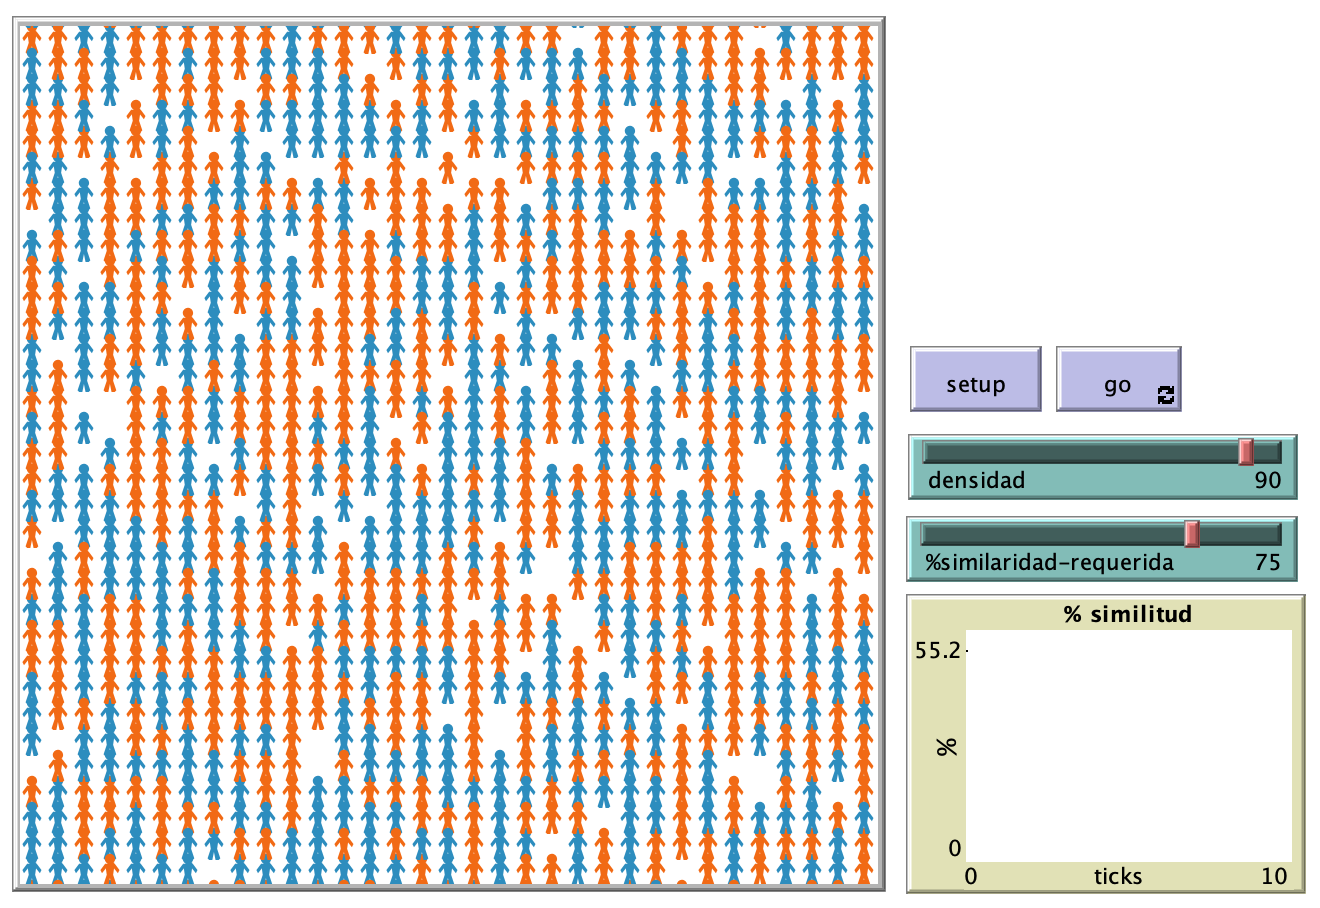
\includegraphics[width=0.7\textwidth]{resources/schelling/01}    
    \caption{\textbf{Setup}, modelo con un valor de densidad igual a 90 y la similiridad de los agentes igual a 75.}
    \label{fig:s-01} 
	\end{figure} 
	
	Al iniciar la ejecución rápidamente los agentes irán alternando su posición dentro de la ventana hasta encontrar una solución; en la ejecución que se muestra en (Fig. \ref{fig:s-02}) se obtiene un resultado exitoso después de 456 ticks.
	
	\begin{figure}[H] 
    \centering
    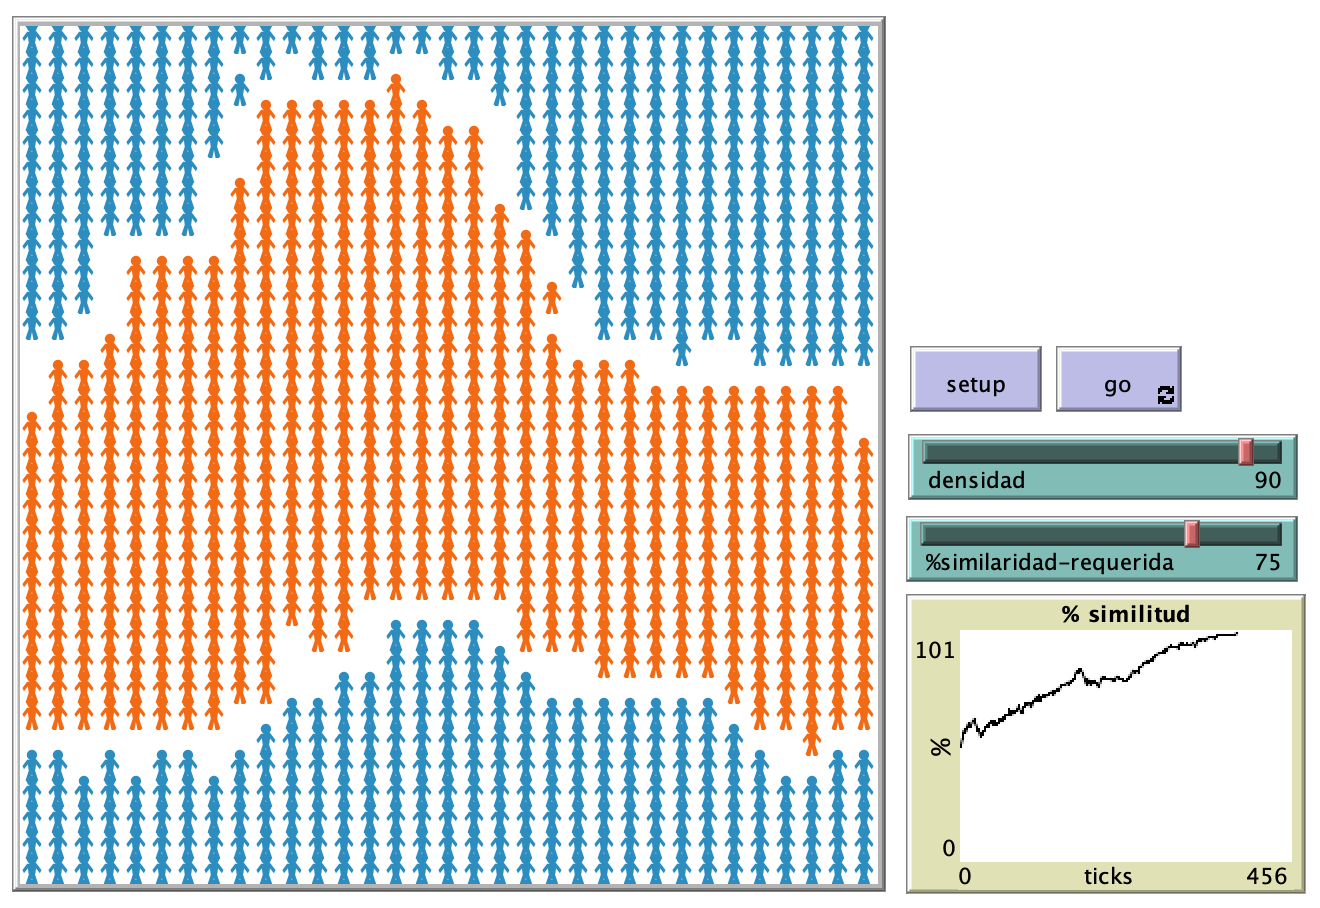
\includegraphics[width=0.7\textwidth]{resources/schelling/02}    
    \caption{\textbf{Go}, modelo con un valor de densidad igual a 90 y la similiridad de los agentes igual a 75.}
    \label{fig:s-02} 
	\end{figure} 
	
	
	\noindent \textbf{Ejecuciones con éxito}
	
	En (Fig. \ref{fig:exito}) se pueden ver cinco ejecuciones donde el modelo converge de manera exitosa. En cuatro de ellas los agentes se segmentan en tres grupos primarios.
	
	% EJEMPLOS CON EXITO
	
	\begin{figure}[h]
    \centering
    \begin{tabular}{ccccc}
        \setlength{\epsfxsize}{0.16\hsize} 
        \subfigure[]{\epsfbox{resources/schelling/05-461}} & 
        \setlength{\epsfxsize}{0.16\hsize} 
        \subfigure[]{\epsfbox{resources/schelling/06-250}} &
        \setlength{\epsfxsize}{0.16\hsize} 
        \subfigure[]{\epsfbox{resources/schelling/07-223}} &
        \setlength{\epsfxsize}{0.16\hsize} 
        \subfigure[]{\epsfbox{resources/schelling/08-836}} &
        \setlength{\epsfxsize}{0.16\hsize} 
        \subfigure[]{\epsfbox{resources/schelling/09-264}} 
    \end{tabular}
    \vspace{-10pt}
    \caption{(a) ejecución en 461 ticks. (b) ejecución en 250 ticks. (c) ejecución en 223 ticks. (d) ejecución en 836 ticks. (e) ejecución en 264 ticks. }
    \label{fig:exito}
	\end{figure}

	
	\noindent \textbf{Ejecuciones sin éxito}

	% EJEMPLOS SIN EXITO
	
	En (Fig. \ref{fig:error}) se pueden ver cinco ejecuciones donde el modelo no converge, los agentes no logran agruparse.
	
\begin{figure}[h]
    \centering
    \begin{tabular}{ccccc}
        \setlength{\epsfxsize}{0.16\hsize} 
        \subfigure[]{\epsfbox{resources/schelling/10}} & 
        \setlength{\epsfxsize}{0.16\hsize} 
        \subfigure[]{\epsfbox{resources/schelling/11}} &
        \setlength{\epsfxsize}{0.16\hsize} 
        \subfigure[]{\epsfbox{resources/schelling/12}} &
        \setlength{\epsfxsize}{0.16\hsize} 
        \subfigure[]{\epsfbox{resources/schelling/13}} &
        \setlength{\epsfxsize}{0.16\hsize} 
        \subfigure[]{\epsfbox{resources/schelling/14}} 
    \end{tabular}
    \vspace{-10pt}
    \caption{El sistema no converge en ninguna prueba, los resultados después de 5,000 ticks se ven de manera similar al punto inicial.}
    \label{fig:error}
\end{figure}

\item  Una propuesta de medida para detectar convergencia es cuando los agentes ya no cambian de posición. Cuándo el parámetro de similitud es igual a Smax, ¿cuál es el tiempo en el que el sistema converge? Realice una gráfica parámetro-similitud vs tiempo-de-convergencia. ¿Cómo crece el tiempo de convergencia en función del parámetro de similitud? ¿lineal, logarítmico, exponencial? Cuando no converja el sistema (probar un tiempo suficientemente grande) dejar de graficar.

Lo primero que debemos hacer es crear un experimento que nos permita extraer los datos a graficar, para esto hacemos uso de la herramienta BehaviorSpace. Se establece como condición de finalización que todos los agentes estén satisfechos conforme al índice de similitud:

\begin{center}
	all? turtles [ satisfecho? ]
\end{center}

El tiempo limite para el experimento será de 5,000 ticks y la densidad del modelo para todas las ejecuciones será de 90\%, igual al problema anterior. Lo que se obtendrá es un archivo de extensión csv que se graficará en MATLAB (Fig. \ref{fig:graph-mat}). 


\begin{figure}[h] 
    \centering
    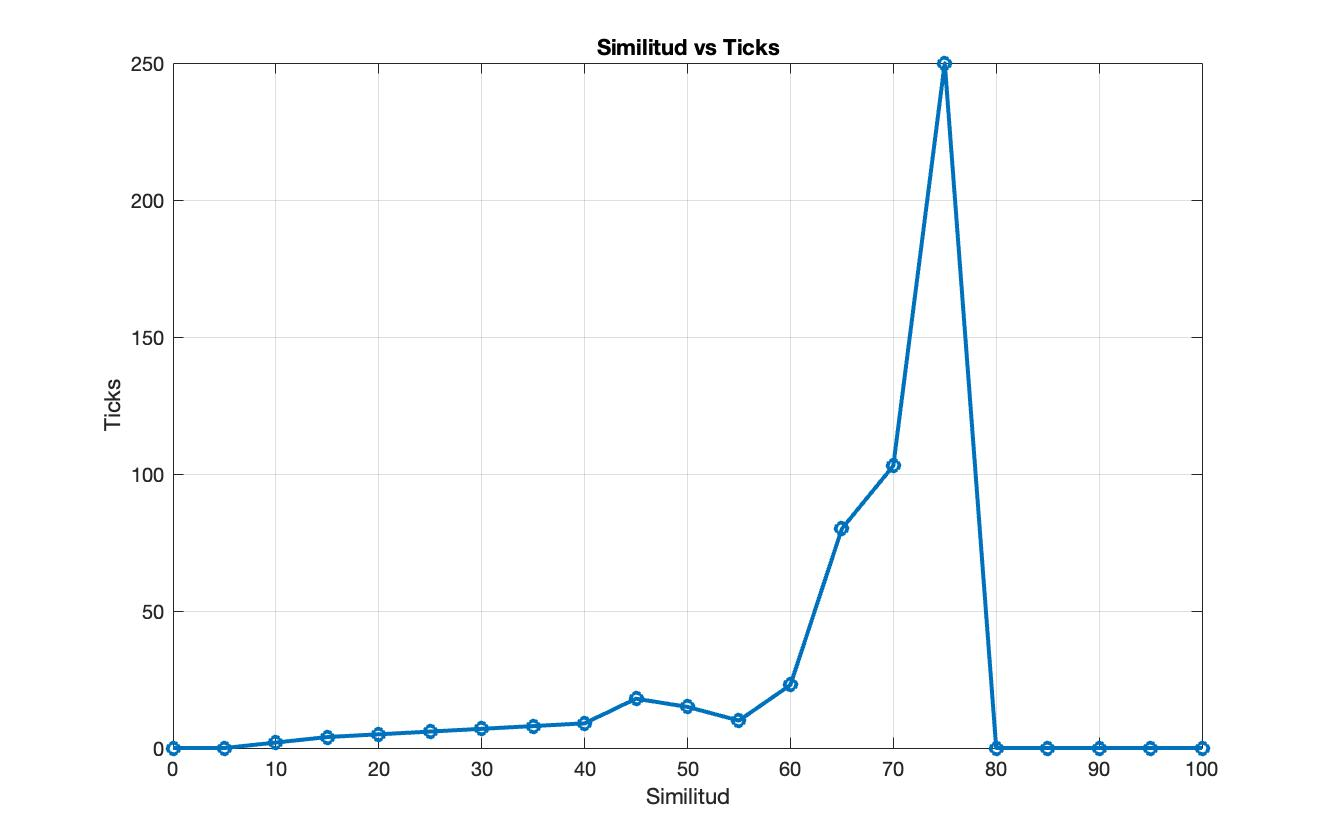
\includegraphics[width=0.7\textwidth]{resources/schelling/grafica}    
    \caption{Gráfica parámetro-similitud vs tiempo-de-convergencia}
    \label{fig:graph-mat} 
	\end{figure} 
	
Para poder visualizarlo mejor, todas la ejecuciones que no se completaron en los 5,000 ticks fueron sustituidas por 0, es por eso que cuando el índice de similitud es mayor a 75 la gráfica desciende abruptamente. El tiempo de convergencia en función del parámetro de similitud crece de manera \textbf{exponencial}. Con lo anterior podemos reafirmar que el valor SMAX es igual a 75.

\item Extensión del modelo. Establezca el parámetro de similitud para cada uno de los agentes, es decir como un atributo del agente. Inicialice la similitud requerida del agente i-ésimo a partir de una distribución normal con media 50 y desviación estándar 10.

Primero para cada agente le agregamos un atributo 'similitud-requerida-agente', dentro de la función  setup y con ayuda de la función generadora asignamos los siguientes parámetros:

	
\begin{verbatim}
set similitud-requerida-agente random-normal 50 10

set similitud-requerida-agente max list 0 min list 100 
	similitud-requerida-agente
\end{verbatim}

\begin{enumerate}
	\item ¿Cómo cambian los patrones de segregación?
	
	En (Fig. \ref{fig:exte}) se puede ver como los agentes se van agrupando en una mayor cantidad de puntos, no solo eso, ya que tienen un patrón menos estricto para la vecindad que los rodea se pueden formar clusters que encapsulen a otros, y es por eso que hay patrones de segregación que contienen en su interior a otros grupos de menor tamaño.
	
	\begin{figure}[H]
    \centering
    \begin{tabular}{ccccc}
        \setlength{\epsfxsize}{0.16\hsize} 
        \subfigure[]{\epsfbox{resources/schelling/15}} & 
        \setlength{\epsfxsize}{0.16\hsize} 
        \subfigure[]{\epsfbox{resources/schelling/16}} &
        \setlength{\epsfxsize}{0.16\hsize} 
        \subfigure[]{\epsfbox{resources/schelling/17}} &
        \setlength{\epsfxsize}{0.16\hsize} 
        \subfigure[]{\epsfbox{resources/schelling/18}} &
        \setlength{\epsfxsize}{0.16\hsize} 
        \subfigure[]{\epsfbox{resources/schelling/19}} 
    \end{tabular}
    \vspace{-10pt}
    \caption{\textbf{Extensión del modelo}}
    \label{fig:exte}
	\end{figure}
	
	\item ¿Qué sucede cuando la media = Smax y la desviación estándar es pequeña o grande?
	
	Cuando la desviación estándar es pequeña los agentes se agrupan pero sin llegar a una solución que finalice el programa (Fig. \ref{fig:peque}). En (Fig. \ref{fig:peque}b) se puede observar como se van agrupando en las esquinas inferior y superior derecha de la ventana y como no logra converger debido a que algunos de los agentes exceden el valor de Smax. 
	
	\begin{figure}[H]
    \centering
    \begin{tabular}{ccccc}
        \setlength{\epsfxsize}{0.40\hsize} 
        \subfigure[]{\epsfbox{resources/schelling/20}} & 
        \setlength{\epsfxsize}{0.40\hsize} 
        \subfigure[]{\epsfbox{resources/schelling/21}} 
 
    \end{tabular}
    \vspace{-10pt}
    \caption{\textbf{media = Smax y la desviación estándar es pequeña} (a) posiciones de inicio (setup). (b) posiciones después de 3,000 ticks.}
    \label{fig:peque}
	\end{figure}
	
	Cuando la desviación estándar es grande los agentes nuevamente se agrupan sin llegar a una solución  (Fig. \ref{fig:grande}). En (Fig. \ref{fig:grande}b) los agentes se concentran en pequeños clusters del centro, pero al igual que en (Fig. \ref{fig:peque}b), algunos de los agentes exceden el valor de Smax y por lo tanto no convergen.
	
	\begin{figure}[H]
    \centering
    \begin{tabular}{ccccc}
        \setlength{\epsfxsize}{0.40\hsize} 
        \subfigure[]{\epsfbox{resources/schelling/22}} & 
        \setlength{\epsfxsize}{0.40\hsize} 
        \subfigure[]{\epsfbox{resources/schelling/23}} 
 
    \end{tabular}
    \vspace{-10pt}
    \caption{\textbf{media = Smax y la desviación estándar es grande} (a) posiciones de inicio (setup). (b) posiciones después de 3,000 ticks.}
    \label{fig:grande}
	\end{figure}

\end{enumerate}

\item Modifique su programa previo para considerar tres tipos de agentes (rojos, verdes y azules). Inicialice cada grupo como 1/3 de la población y establezca de manera global el parámetro de similitud-requerida.

	Primero hay que realizar las modificaciones en el modelo para colorear de verde a los agentes (en este caso su color es 45). Como el color se debe distribuir de manera uniforme, lo que se hace es dividir el número de agentes entre tres, su residuo puede ser 0, 1 o 2 y en base a eso se asigna un color. El código de 'setup' queda de la siguiente forma:
	
\begin{verbatim}
to setup
  clear-all
  let colores [25 55 95]  
  let num-agentes 0
  ask patches [
    set pcolor white
    if random 100 < densidad [
      sprout 1 [
        set color item (num-agentes mod 3) colores 
        set size 1.3
        set shape "person"
        set num-agentes num-agentes + 1  
      ]
    ]
  ]
  actualizar-tortugas
  actualizar-variables
  reset-ticks
end
\end{verbatim}


\begin{itemize}
	\item  ¿Se forman patrones de segregación?
	
	Haciendo pruebas cuando la densidad del modelo es igual a 90 se obtienen patrones de segregación bien delimitados. En (Fig. \ref{fig:exteTres11}) se observan cinco pruebas del modelo. En promedio se obtienen siete clusters de formas irregulares. 
	
	\begin{figure}[H]
    \centering
    \begin{tabular}{ccccc}
        \setlength{\epsfxsize}{0.16\hsize} 
        \subfigure[]{\epsfbox{resources/schelling/25}} & 
        \setlength{\epsfxsize}{0.16\hsize} 
        \subfigure[]{\epsfbox{resources/schelling/26}} &
        \setlength{\epsfxsize}{0.16\hsize} 
        \subfigure[]{\epsfbox{resources/schelling/27}} &
        \setlength{\epsfxsize}{0.16\hsize} 
        \subfigure[]{\epsfbox{resources/schelling/28}} &
        \setlength{\epsfxsize}{0.16\hsize} 
        \subfigure[]{\epsfbox{resources/schelling/29}} 
    \end{tabular}
    \vspace{-10pt}
    \caption{\textbf{Extensión del modelo a tres tipos de agentes}. La ejecución más rápida finalizó con 205 ticks y la más lenta con 600.}
    \label{fig:exteTres11}
	\end{figure}
	
	\item  ¿Cuál es el valor del umbral Smax?
	
	Análogo al primer punto de la práctica, de manera empírica se prueba cambiando el valor de similitud cuando la densidad es 90. Con esto se obtiene que el \textbf{Smax es igual a 62}, cuando es sustituido por 63 el modelo no converge (Fig. \ref{fig:exteTres12}).
	
		\begin{figure}[H]
    \centering
    \begin{tabular}{ccccc}
        \setlength{\epsfxsize}{0.16\hsize} 
        \subfigure[]{\epsfbox{resources/schelling/30}} & 
        \setlength{\epsfxsize}{0.16\hsize} 
        \subfigure[]{\epsfbox{resources/schelling/31}} &
        \setlength{\epsfxsize}{0.16\hsize} 
        \subfigure[]{\epsfbox{resources/schelling/32}} &
        \setlength{\epsfxsize}{0.16\hsize} 
        \subfigure[]{\epsfbox{resources/schelling/33}} &
        \setlength{\epsfxsize}{0.16\hsize} 
        \subfigure[]{\epsfbox{resources/schelling/34}} 
    \end{tabular}
    \vspace{-10pt}
    \caption{\textbf{Extensión del modelo a tres tipos de agentes}. La ejecución más rápida finalizó con 205 ticks y la más lenta con 600.}
    \label{fig:exteTres12}
	\end{figure}
	
\end{itemize} 
	
\item Bajo su criterio que otros elementos de modelación se podrían definir en el modelo de Schelling para hacerlo más realista.  ¿Qué otros análisis podrían implementar para explicar las dinámicas

Se podría modificar el índice de similitud tal que agentes de diferentes 'clases', en este caso colores, tengan diferentes valores. De esta manera el modelo podría dar como resultado segregaciones menos rígidas para unos agentes. También se puede acotar la sección en la que pueden rotar los elementos. Se podrían analizar 

\end{enumerate}
\section{Termitas apiladoras}

\begin{enumerate}
	\item Implemente el modelo de termitas apiladoras, pueden usar el código visto en clase o lo pueden programan en otro lenguaje de programación. 
	
	Se toma la implementación vista en clase como referencia para el desarrollo de este apartado de la práctica, definiendo variables que faciliten la graficación, el coloreado de los agentes y la escalabilidad del modelo. La implementación vista en clase se puede consultar en el archivo 'Termitas-01.nlog', en (Fig. \ref{fig:termitasApiladoras01}) se pueden ver ejemplos de cinco ejecuciones.
	
	
	\begin{figure}[H]
    \centering
    \begin{tabular}{ccccc}
        \setlength{\epsfxsize}{0.16\hsize} 
        \subfigure[]{\epsfbox{resources/termitas/01}} & 
        \setlength{\epsfxsize}{0.16\hsize} 
        \subfigure[]{\epsfbox{resources/termitas/02}} &
        \setlength{\epsfxsize}{0.16\hsize} 
        \subfigure[]{\epsfbox{resources/termitas/03}} &
        \setlength{\epsfxsize}{0.16\hsize} 
        \subfigure[]{\epsfbox{resources/termitas/04}} &
        \setlength{\epsfxsize}{0.16\hsize} 
        \subfigure[]{\epsfbox{resources/termitas/05}} 
    \end{tabular}
    \vspace{-10pt}
    \caption{\textbf{Termitas apiladoras}. La población es igual a 77 y su densidad es 17.}
    \label{fig:termitasApiladoras01}
	\end{figure}
	
	\item Implemente dos gráficas donde se observe el comportamiento del sistema en función del tiempo.
	
	\begin{figure}[h] 
    \centering
    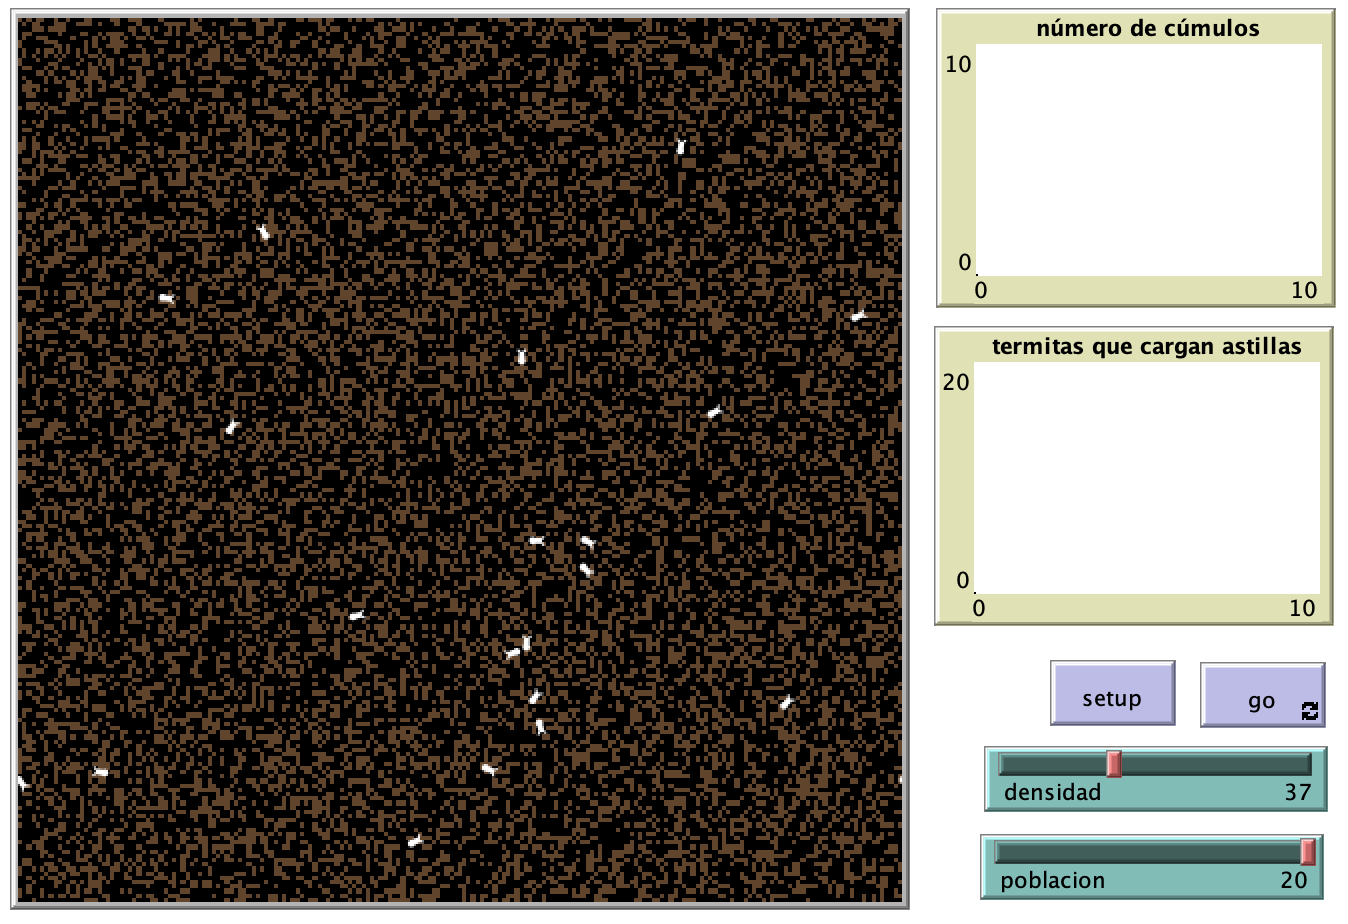
\includegraphics[width=0.7\textwidth]{resources/termitas/06}    
    \caption{Implementación de ambas gráficas en el modelo de termitas apiladoras.}
    \label{fig:termitas-dos} 
	\end{figure} 
	
	
	
	\begin{itemize}
		\item el número de cúmulos en función del tiempo
		
		Se define una variable global \textbf{cumulos}, dentro de la función \textbf{go} se incrementa una unidad a esta variable siempre y cuando se cumpla la siguiente propiedad:
		
		\begin{verbatim}
ask patches [
	if tipo != 0 and visitado = false [
        recorrer-cumulo
        set cumulos cumulos + 1
    ]
]
		\end{verbatim}
		
		En \textbf{recorrer-cumulo} si el patch tiene madera y aún no ha sido visitado entocnes el patch se etiqueta como verdadero. Dada una vecindad de ocho, si uno de los patch tiene presencia de madera y no ha sido visitado entonces continúa (Fig. \ref{fig:001}).
		
	\begin{figure}[H]
    \centering
    \begin{tabular}{ccccc}
        \setlength{\epsfxsize}{0.40\hsize} 
        \subfigure[]{\epsfbox{resources/termitas/07}} & 
        \setlength{\epsfxsize}{0.40\hsize} 
        \subfigure[]{\epsfbox{resources/termitas/08}} 
 
    \end{tabular}
    \vspace{-10pt}
    \caption{(a) Comportamiento de la gráfica en 78,100 ticks cuando el valor de densidad es igual 37 y la población es 20. (b) cómo está implementado el plot.}
    \label{fig:001}
	\end{figure}
		
		\item el número de termitas que están cargando astillas

		Dentro de la función buscar madera los agentes cambian su color a naranja, esto sirve para graficar el número de termitas cargando astillas (Fig. \ref{fig:002}), basta con modificar el valor de la pluma de la gráfica de la siguiente manera:
		\begin{verbatim}
			plot count turtles with [color = orange]
		\end{verbatim}
		
			\begin{figure}[H]
    \centering
    \begin{tabular}{ccccc}
        \setlength{\epsfxsize}{0.40\hsize} 
        \subfigure[]{\epsfbox{resources/termitas/09}} & 
        \setlength{\epsfxsize}{0.40\hsize} 
        \subfigure[]{\epsfbox{resources/termitas/10}} 
 
    \end{tabular}
    \vspace{-10pt}
    \caption{(a) Comportamiento de la gráfica en 78,100 ticks cuando el valor de densidad es igual 37 y la población es 20. (b) cómo está implementado el plot.}
    \label{fig:002}
	\end{figure}
		
		
		
	
	\end{itemize}
	
	
	

\end{enumerate}

\bibliographystyle{plain}
\bibliography{references.bib}

\end{document}